\documentclass[tikz,border=5pt]{standalone}

\usepackage{pgfplots}
\pgfplotsset{compat=1.18}

\definecolor{mygrey}{RGB}{150,150,150}
\definecolor{mygreen}{RGB}{76,175,80}

\begin{document}

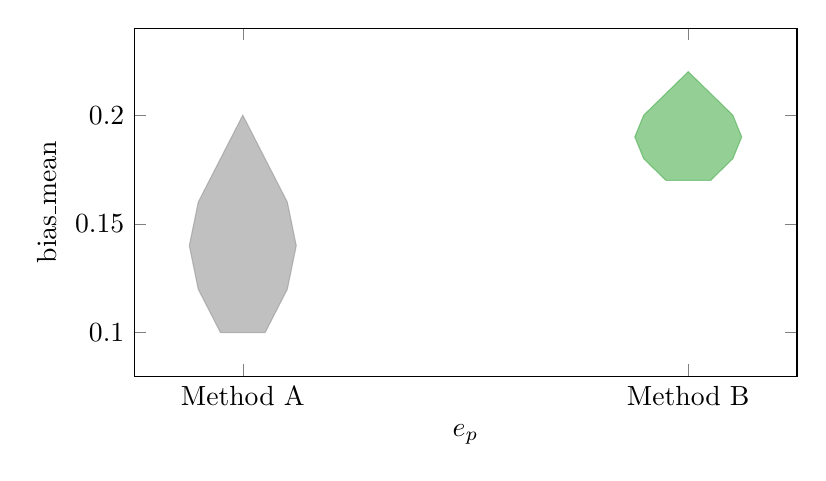
\begin{tikzpicture}

\begin{axis}[
    width=10cm,
    height=6cm,
    xlabel={$e_p$},
    ylabel={bias\_mean},
    xtick={1,2},
    xticklabels={Method A, Method B},
    ymin=0.08, ymax=0.24,
]

% --- Grey violin (mirrored density) ---
\addplot[
    fill=mygrey,
    draw=mygrey,
    opacity=0.6
] coordinates {
(1-0.05,0.10)
(1-0.10,0.12)
(1-0.12,0.14)
(1-0.10,0.16)
(1-0.05,0.18)
(1,0.20)
(1+0.05,0.18)
(1+0.10,0.16)
(1+0.12,0.14)
(1+0.10,0.12)
(1+0.05,0.10)
} -- cycle;

% --- Green violin ---
\addplot[
    fill=mygreen,
    draw=mygreen,
    opacity=0.6
] coordinates {
(2-0.05,0.17)
(2-0.10,0.18)
(2-0.12,0.19)
(2-0.10,0.20)
(2-0.05,0.21)
(2,0.22)
(2+0.05,0.21)
(2+0.10,0.20)
(2+0.12,0.19)
(2+0.10,0.18)
(2+0.05,0.17)
} -- cycle;

\end{axis}

\end{tikzpicture}

\end{document}
